\chapter{Mitarbeiter}
\label{mitarbeiter}
\begin{figure}
	\centering
	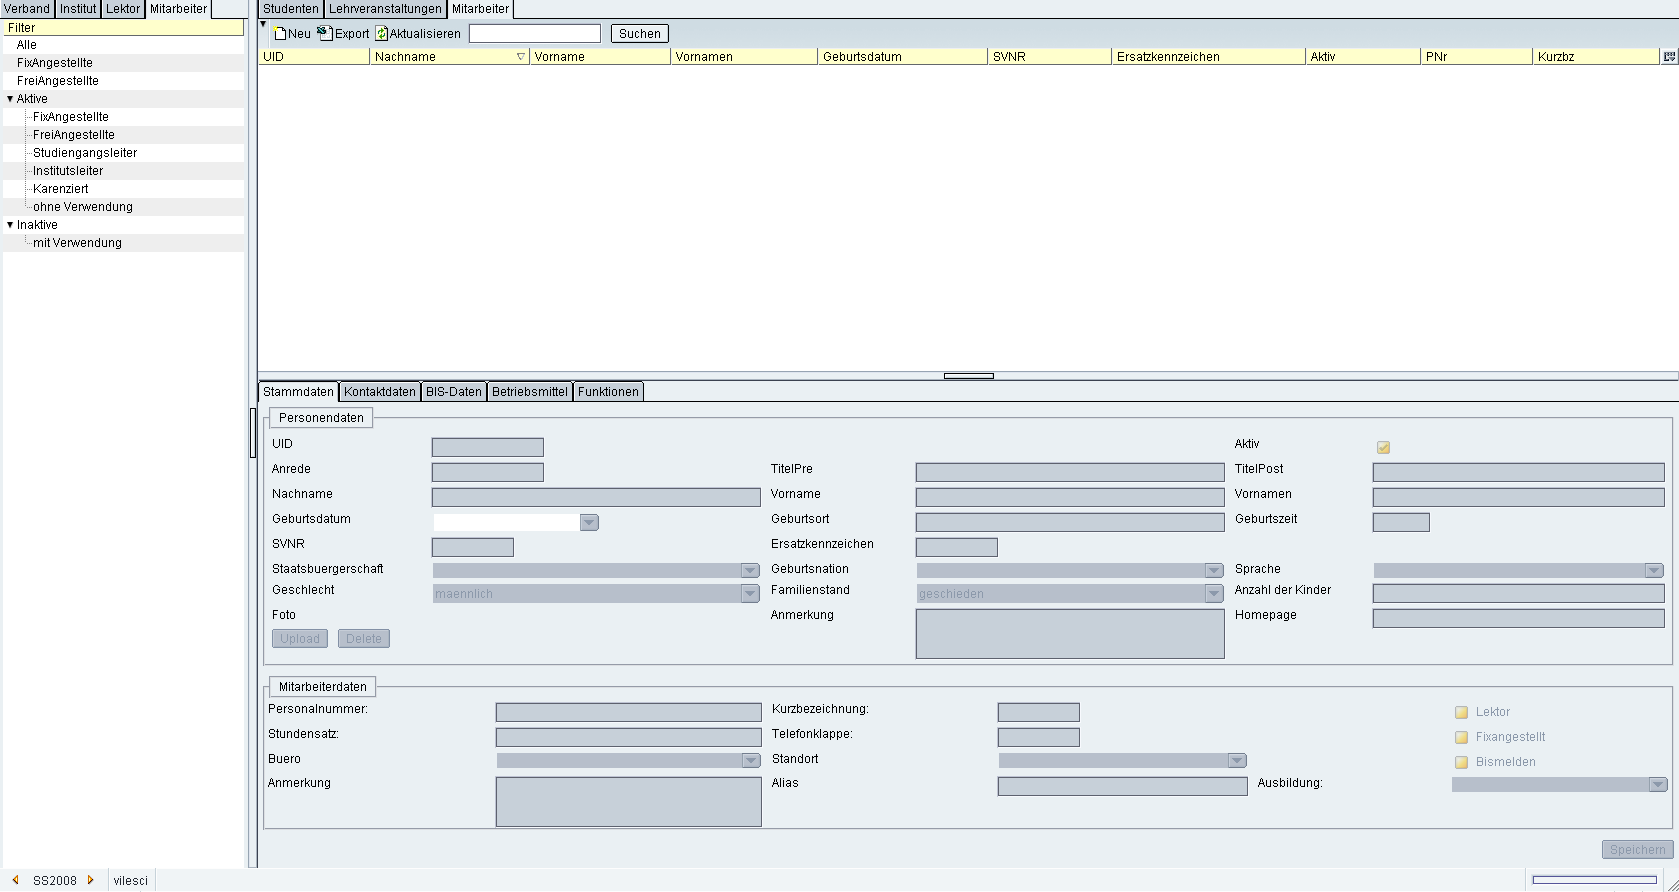
\includegraphics[width=0.75\textwidth]{FAS_Mitarbeiter2.png}
	\caption{Ansicht Mitarbeiterbereich}
	\label{Mitarbeiter2}
\end{figure}
\section{Anzeigefilter}
\begin{itemize}
	\item Alle: Es werden im Listenfeld 2 alle Mitarbeiter ohne Einschr�nkungen angezeigt.
	\item FixAngestellte: Es werden alle Mitarbeiter angezeigt, bei denen \textit{Fixangestellt} (in der Karteikarte \textit{Stammdaten} der Mitarbeiter rechts unten) angehakt ist. 
	\item FreiAngestellte: Es werden alle Mitarbeiter angezeigt, bei denen \textit{Fixangestellt} (in der Karteikarte \textit{Stammdaten} der Mitarbeiter rechts unten) nicht angehakt ist.
	\item Aktive: Die nachfolgenden Filter listen nur Mitarbeiter auf, die als aktiv (in der Karteikarte \textit{Stammdaten} der Mitarbeiter rechts oben) gekennzeichnet sind.
	\begin{itemize}
		\item FixAngestellte: wie FixAngestellte unter \textit{Alle}, aber hier nur aktive Mitarbeiter.
		\item FreiAngestellte: wie FreiAngestellte unter \textit{Alle}, aber hier nur aktive Mitarbeiter.
		\item Karenziert: Es werden hier aktive Mitarbeiter aufgelistet, bei denen eine aktuelle Verwendung (unter Karteikarte \textit{BIS-Daten}) mit Ausmass \textsl{Karenz} eingegeben ist.
		\item Ohne Verwendung: Es werden alle aktiven Mitarbeiter aufgelistet, bei denen keine aktuelle Verwendung eingetragen ist.
		\item Studiengangsleiter: Es werden alle aktiven Mitarbeiter, bei denen zumindest eine Funktion \textit{Leitung} f�r einen Studiengang in der Karteikarte \textit{Funktionen} eingetragen ist.
		\item Institutsleiter: Es werden alle aktiven Mitarbeiter, bei denen zumindest eine Funktion \textit{Leitung} f�r ein Institut in der Karteikarte \textit{Funktionen} eingetragen ist.
	\end{itemize}
	\item Inaktive: Es werden im Listenfeld 2 alle Mitarbeiter angezeigt, die nicht als aktiv (in der Karteikarte \textit{Stammdaten} der Mitarbeiter rechts oben) gekennzeichnet sind. 
	\begin{itemize}
		\item Mit Verwendung: Hier werden Mitarbeiter aufgelistet, die nicht als aktiv gekennzeichnet sind, aber dennoch eine aktuelle Verwendung besitzen.
	\end{itemize}
\end{itemize}
\section{Mitarbeiterdatenkarten}
\subsection{Stammdaten}
Die Karteikarte \textit{Stammdaten} beinhaltet die Personen- und Mitarbeiterdaten des in Listenfeld 2 ausgew�hlten  Mitarbeiters. Besonders zu beachten sind die vier Checkboxen auf dieser Seite:
\begin{itemize}
	\item Aktiv: Diese Checkbox entscheidet ob der Mitarbeiter als aktiv gef�hrt wird. Eine Woche nach der Entfernung des H�kchens wird der Mitarbeiter �ber die Deaktivierung seines Accounts informiert. Der Account wird dann ein Jahr sp�ter nach einem weiteren Benachrichtigungsmail gel�scht.
	\item Lektor: Diese Checkbox mu� markiert sein, damit der Mitarbeiter einer Lehreinheit als Unterrichtender zugewiesen werden kann.
	\item Fixangestellt: Diese Checkbox unterscheidet Mitarbeiter mit einem fixen Arbeitsvertrag von Mitarbeitern mit einem freien Dienstverh�ltnis und wirkt sich auf die Mailverteiler und die Filter der Mitarbeiterverwaltung aus.
	\item Bismelden: Ist diese Checkbox markiert, wird der Mitarbeiter in die BIS-Meldung einbezogen.
\end{itemize}
\subsection{Kontaktdaten}
Die Karteikarte \textit{Kontaktdaten} beinhaltet die Adresse, die E-Mailadresse, Telefon- und Faxverbindungen sowie die Bankverbindungen des Mitarbeiters. Diese Karteikarte entspricht in Aufbau und Funktion der Karteikarte \textit{Kontakt} der Studenten (siehe Kapitel \ref{kontakte}).
\subsection{BIS-Daten}
\begin{figure}
	\centering
	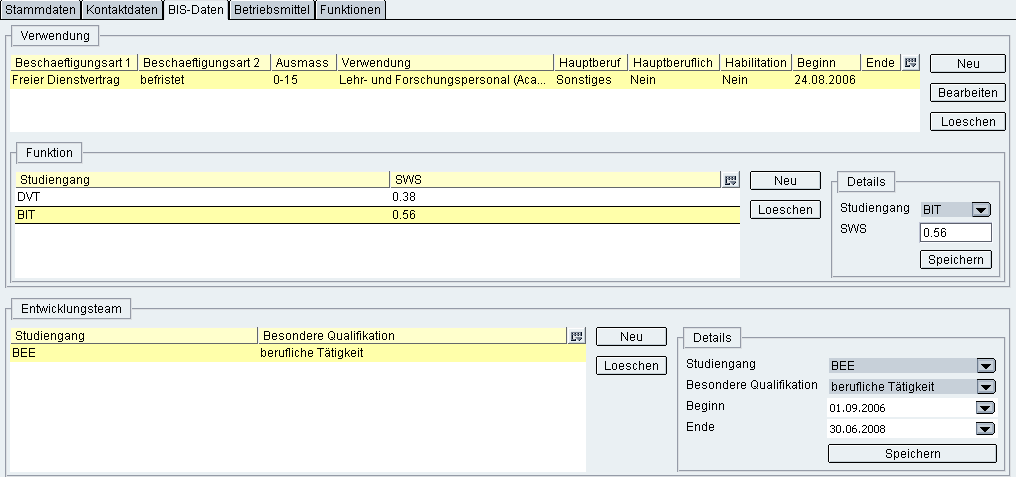
\includegraphics[width=0.75\textwidth]{FAS_BISDaten1.png}
	\caption{BIS-Daten}
	\label{BISDaten1}
\end{figure}
Abbildung \ref{BISDaten1} zeigt die Karteikarte \textit{BIS-Daten}, mit der die BIS-Daten der Mitarbeiter bearbeitet werden. Die Karteikarte besteht aus drei Teilen:
\begin{enumerate}
	\item Verwendung: Die Verwendung des Mitarbeiters ist eine Abbildung des Dienstvertrages.\\
	Der \textit{Verwendung}-Bereich ist ein Listenfeld, das die vergangenen und gegenw�rtigen Verwendungen des Mitarbeiters anzeigt. Mit der Taste \textit{Neu} �ffnet sich ein Eingabefenster mit leeren Eingabefenstern zum Anlegen einer neuen Verwendung. Wird eine Verwendung markiert, kann mit einem Klick auf den Button \textit{Bearbeiten} diese Verwendung ver�ndert werden oder mit einem Klick auf den Button \textit{Loeschen} entfernt werden. \\
	Das Eingabeformular besteht aus folgenden Eingabe- und Auswahlfeldern:
	\begin{itemize}
		\item Beschaeftigungsart 1: Art des Dienstvertrags. In den meisten F�llen \textsl{Echter Dienstvertrag} oder \textsl{Freier Dienstvertrag}
		\item Beschaeftigungsart 2: Auswahl, ob der Dienstvertrag unbefristet oder befristet ist.
		\item Beschaeftigungsausmass: F�r jede einer Person zugewiesenen Kategorie der Besch�ftigungsart 1 (Vertragstypen) ist das entsprechende Besch�ftigungsausma� anhand folgender Einteilung anzugeben.\\
		Das Besch�ftigungsausma� ist definiert als die auf den Berichtszeitraum (12 Monate) umgerechnete Wochenarbeitszeit je Besch�ftigungsverh�ltnis einer Person.
		\begin{table*}
			\centering
				\begin{tabular}{|c|c|}
					\hline
					BeschAusmassCode&BeschAusmassBez\\
					\hline
					1&Vollzeit\\
					\hline
					2&<=15 Wochenstunden\\
					\hline
					3&16-25 Wochenstunden\\
					\hline
					4&26-35 Wochenstunden\\
					\hline
					5&Karenz\\
					\hline
				\end{tabular}
			\caption{BIS - Beschaeftigungsausmass}
			\label{tab:BIS - Beschaeftigungsausmass}
		\end{table*}
		(BIS Schnittstelle Version 5.1, 20.10.2006, FHR)
		\item Verwendung: Mitarbeiter m�ssen einer Verwendungsgruppe zugeordnet werden. Siehe Tabelle \ref{tab:BIS - Verwendung}
		\begin{table*}
			\centering
				\begin{tabular}{|c|c|}
					\hline
					Verwendungscode&VerwendungBez\\
					\hline
					1&Lehr- und Forschungspersonal\\
					&(Academic staff)\\
					\hline
					2&Lehr- und Forschungshilfspersonal\\
					&(Teaching and Research assistants)\\
					\hline
					3&Akademische Dienste f�r Studierende\\
					&(Academic Support)\\
					\hline
					4&Soziale Dienste und Gesundheitsdienste\\
					&(Health and Social Support)\\
					\hline
					5&Studiengangsleiter/in\\
					\hline
					6&Leiter/in FH-Kollegium\\
					\hline
					7&Management\\
					&(School Level Management))\\
					\hline
					8&Verwaltung\\
					&(School Level Administrative Personnel)\\
					\hline
					9&Hauspersonal, Geb�ude-/Haustechnik\\
					&(Maintenance and Operations Personnel)\\
					\hline
				\end{tabular}
			\caption{BIS - Verwendung}
			\label{tab:BIS - Verwendung}
		\end{table*}
		\item Hauptberuflich Lehrende(r): Anzugeben ist, ob es sich um eine/n hauptberuflich Lehrende/n handelt.\\
		Die Angabe \"haupts�chlich Lehrende/r - ja\" ist nur bei den Verwendungscodes 1 (Lehr- und Forschungspersonal), 5 (Studiengangsleiter/in) und 6 (Leiter/in FH-Kollegium) m�glich. F�r die Definition des/der hauptberuflich Lehrenden sind folgende Kriterien relevant: das zeitliche Ausma� der T�tigkeit, der Anteil an den Eink�nften und die Art der T�tigkeit (Profil). (BIS Schnittstelle Version 5.1, 20.10.2006, FHR)
		\item Hauptberuf: Bei nebenberuflich Lehrenden ist die deren Hauptberuf anzugeben und einer Hauptberufkategorie zuzuordnen.
		\item Habilitation
		\item Beginn: Beginndatum der Verwendung.
		\item Ende: Endedatum der Verwendung.
		\item Vertragsstunden: Vertraglich vereinbarte Arbeitsstunden. Dieser Wert wird nicht direkt in der BIS-Meldung verwendet.
	\end{itemize}
	\item Funktion:\\
	In diesem Bereich werden Lehrfunktionen des ausgew�hlten Mitarbeiters festgehalten. Die Eingabe startet mit einem Klick auf den Button \textit{Neu}, dann k�nnen der Studiengang ausgew�hlt und die Semesterwochenstunden (SWS) eingegeben werden.\\
	Mit dem Button \textit{Loeschen} k�nnen markierte Eintr�ge von Funktionen gel�scht werden.
	\item Entwicklungsteam: \\
	In diesem Bereich wird angegeben, ob der Mitarbeiter im Entwicklungsteam von Studieng�ngen war und welche Qualifikation daf�r ausschlaggebend war.
\end{enumerate}
\subsection{Betriebsmittel}
Hier werden die entliehenen Betriebsmittel wie z.B. Schl�ssel festgehalten (siehe Kap. \ref{betriebsmittel}).
\subsection{Funktionen}
In dieser Karteikarte werden die Funktionen der Mitarbeiter, und in welchem Studiengang und Institut diese ausge�bt werden, festgehalten. 
Der Aufbau dieser Karteikarte wird in Kapitel \ref{funktionen} beschrieben.
\section{Neuen Mitarbeiter anlegen}
\begin{figure}
	\centering
	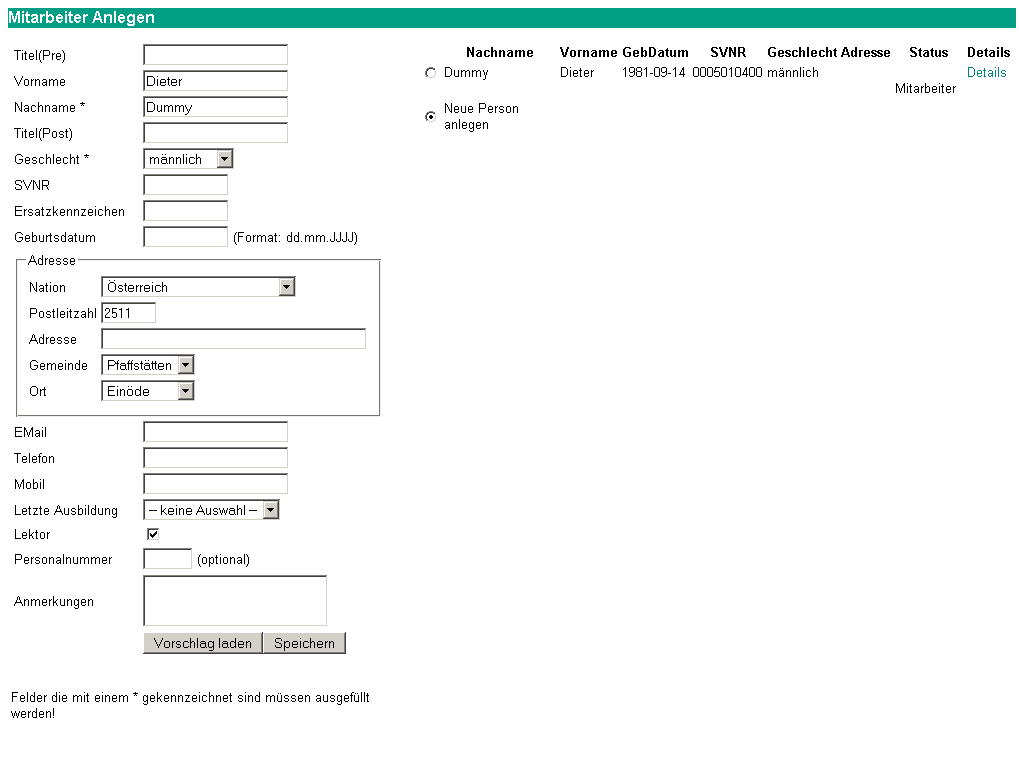
\includegraphics[width=0.75\textwidth]{FAS_Mitarbeiter1.png}
	\caption{Neuen Mitarbeiter anlegen}
	\label{Mitarbeiter1}
\end{figure}
Um einen neuen Mitarbeiter anzulegen, mu� entweder im Listenfeld 1 oder im Listenfeld 2 auf den Karteireiter \textit{Mitarbeiter} geklickt und danach in der Men�leiste des Listenfeld 2 der Button \textit{Neu} angeklickt werden. Dadurch �ffnet sich die in Abbildung \ref{Mitarbeiter1} gezeigte Eingabemaske. Nach der Eingabe der Mitarbeiterdaten und einem klick auf 'Vorschlag laden' wird gepr�ft, ob diese Person bereits im System vorhanden ist. Wenn die gew�nschte Person in der Liste aufscheint, klicken Sie auf den kleinen Kreis neben der Person. Andernfalls w�hlen Sie den Punkt 'Neue Person anlegen' aus. Der Mitarbeiter wird danach mittels \textit{Speichern}-Taste in die Datenbank �bertragen.

